\section{\color{red}Andre datastrukturer}
\subsection{Heap (prioritetskø)}
En heap (også kalt prioritetskø) er en type binært tre med noen spesielle struktur- og ordningskrav. Vi har to typer heap: min- og maksheap. Vi vil beskrive minheap i dette kapitlet, men maksheap fremgår helt analogt.

\begin{definisjon} En minheap er et binært tre der følgende krav er oppfylt:  \label{def:heap}
\begin{enumerate}
\item Treet er komplett (høyden til treet er $ \lceil\log_2 n\rceil $)
\item En node har alltid (sorterings)verdi mindre enn, eller lik sine barn. 
\end{enumerate}
\end{definisjon}

En maksheap defineres nesten likt, eneste forskjell er at pt. 2 i definisjonen blir ``En node alltid er større enn, eller lik sine barn.''

Hver node i en heap inneholder to ting: et element, og en verdi vi sorterer etter. I motsetning til i et binært søketre der vi sorterer på elementet selv, vil vi med en heap tilordne en sorteringsverdi til hvert element som ikke trenger å ha noe med elementet å gjøre. 

~\\
\begin{figure}[H]
\centering
\caption{En (min)heap. For oversiktens skyld er kun sorteringsverdiene tatt med.}
\label{fig:heap}
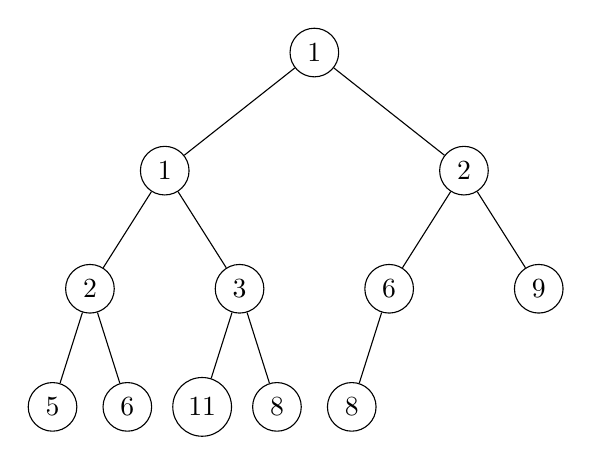
\begin{tikzpicture}[level distance=1.5cm,
  level 1/.style={sibling distance=3.8cm},
  level 2/.style={sibling distance=1.9cm},
  level 3/.style={sibling distance=0.95cm},
every node/.style = {shape=circle, draw, align=center}]

\node{1}
	child {node {1}
		child {node {2}
			child {node {5}}
			child {node {6}}
		}
		child {node {3}
			child {node {11}}
			child {node {8}}
		}
	}
	child {node {2}
		child {node {6}
			child {node {8}}
			child [missing] {}
		}
		child {node {9}}
	};
\end{tikzpicture}
\end{figure}

\paragraph{Innsetting}~\\
Når vi skal sette inn et element i en heap setter vi den på første ledige plassen. Deretter sammenligner vi nodens verdi med forelderens verdi. Hvis forelderen har større verdi enn noden vi setter inn bytter vi plass\footnote{Foreleser og lærebok kaller denne prosessen \say{percolate up}}. Så sammenligner vi med den nye forelderen, bytter plass om nødvendig, og fortsetter slik til enten forelderen er mindre enn noden, eller at noden er rot. 

\paragraph{Fjerning (deleteMin)}~\\
I en heap er vi egentlig bare interessert i å ta ut det minste elementet fra en heap (hvorfor blir diskutert i avsnittet om anvendelser). På grunn av krav 2 i definisjonen vet vi at rota er det minste elementet i heapen. Derfor fjerner vi rota. For å skaffe en ny rot tar vi det siste elementet i heapen og setter som rot. Deretter sammenligner vi verdien av den nye rota med verdien av barna. Hvis et (eller begge) av barna har mindre verdi enn den nye rota bytter rota plass med \textbf{det minste} barnet\footnote{\say{percolate down}}. Vi fortsetter slik til ordningskravet er oppfylt (noden har mindre verdi enn barna). 

\paragraph{Implementasjon}~\\
Vi kan implementere en heap som et tre (dvs, lage nodeobjekter med pekere til barn etc), men som oftest implementerer vi en heap ved hjelp av en array. Vi lar rota være på index 1. På grunn av kompletthetskravet kan vi legge nodene radvis bak rota. Vi finner da barna til en node på index $ i $ ved å til index $ 2i $ (venstre barn) og $ 2i+1 $ (høyre barn), og forelder ved å gå til index $ \lfloor i/2 \rfloor $. Når vi implementerer en heap som en array kan vi risikere å gå tom for plass i arrayen. Da må vi lage en ny array, og flytte over alle elementene til den nye arrayen. Vanligvis legger vi til en og en rad i slengen (eventuelt to og to, tre og tre, etc..). Å gjøre dette tar åpenbart $ O(n) $ tid, men vi må gjøre det sjeldnere og sjeldnere jo større heapen blir. 

\begin{figure}[H]
\centering
\caption{Heapen i fig \ref{fig:heap} representert som array}
\begin{tabular}{r||c|c|c|c|c|c|c|c|c|c|c|c|c|c|c|c}
	~~index &  0   & 1 & 2 & 3 & 4 & 5 & 6 & 7 & 8 & 9 & 10 & 11 & 12 &  13  &  14  &  15  \\ \hline
	~~verdi & null & 1 & 1 & 2 & 2 & 3 & 6 & 9 & 5 & 6 & 11 & 8  & 8  & null & null & null 
\end{tabular}
\end{figure}

I Java har vi en ferdig heap: \verb|java.util.PriorityQueue<E>|. Java krever at \verb|E| er sammenlignbar med seg selv (\verb|E| implementerer \verb|comparable<E>|) og vil bruke den sammenligningen som grunnlag for sortering. Javas heap er implementert som array. 

\paragraph{Tidsanalyse}~\\
Vi ser på kjøretiden til de to omtalte operajonene:
\begin{teorem} Kjøretid for heapoperasjoner \label{teo:heapop}
\begin{enumerate}[i]
\item Innsetting i en heap tar $ O(\log_2 n) $ tid
\item Fjerne minste element tar $ O(\log_2 n) $ tid
\end{enumerate}
\end{teorem}
Beviset følger av strukturkravet i definisjon \ref{def:heap}:
\begin{bevis} Teorem \ref{teo:heapop}, del i:

Når vi setter inn et element i en heap må vi først sette elementet på slutten av heapen. Siden vi vet hvor siste element er vil dette ta $ O(1) $ tid. Deretter må vi justere plassen til elementet ved å la elementet sive oppover. Siden treet er komplett vil høyden på treet være $ \lceil\log_2 n\rceil $, og vi kan maksimalt foreta $ \lceil\log_2 n\rceil - 1 $ byttinger. Total tid blir derfor være $ O(\log_2 n) $
\end{bevis}
Argumentet for teo. \ref{teo:heapop}, del ii er helt analogt. 


\paragraph{Anvendelser}~\\
I dette kurset ser vi på to anvendelser av en heap: Prioritetskø og sortering. Når vi bruker en (min)heap som en prioritetskø lar vi viktige jobber ha lav verdi, og mindre viktige jobber ha høy verdi. Når vi jobbene våre inn i en heap og tar dem ut vil de viktigste jobbene komme først.

Vi kan også sortere en liste med elementer ved hjelp av en heap. Se \ref{heapsort}.



\subsubsection{Venstreorientert (leftist) heap}
En venstreorientert heap er en en heap med et annet strukturkrav enn vanlig heap. Motivasjonen bak venstreorienterte heaper er at å flette (merge) to heaper av samme størrelse tar $ O(n) $ tid, vi ønsker å forbedre det. Før vi kan definere en venstreorientert heap må vi definere \say{null path length} (herfra: npl). Npl til en node $ n $ er lengden av den korteste veien fra $ n $ til en etterkommer uten to barn ($ 0 $ hvis $ n $ har $ <2 $ barn). 

\begin{definisjon} En venstreorientert heap er et binært tre der følgende krav er oppfylt:
\begin{enumerate}
\item For hver node $ n $ i treet er $ \text{npl}(l) \geq \text{npl}(r) $, der $ l $ er venstre og $ r $ er høyre barn til $ n $.
\item En node har alltid (sorterings)verdi mindre enn, eller lik sine barn. 
\end{enumerate}
\end{definisjon}

\begin{figure}[H]
\centering
\caption{Et tre med $ \text{npl}(n) $ skrevet inn}
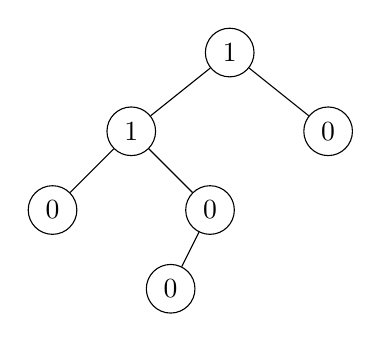
\begin{tikzpicture}[level distance=1cm,
  level 1/.style={sibling distance=2.5cm},
  level 2/.style={sibling distance=2cm},
  level 3/.style={sibling distance=1cm},
every node/.style = {shape=circle, draw, align=center}]

\node{1}
child {
	node {1}
	child {
		node {0}
	}
	child {
		node {0}		
		child {
			node {0}
		}
		child[missing]
	}
}
child {
	node {0}
};
\end{tikzpicture}
\end{figure}

\noindent \textbf{Merk:} En venstreorientert heap forsøker å være ute av balanse.

\paragraph{Operasjoner}~\\
Hovedoperasjonen på venstreorienterte heaper er \textbf{fletting} (engelsk: merging). Vi kan implementere fletting rekursivt: Når vi skal flette to heaper $ H_1 $ og $ H_2 $ sammenligner vi først røttene. La $ H_1 $ være heapen med minst rot. La så den høyre subheapen til $ H_1 $ være heapen som fremstår ved å flette høyre subheap i $ H_1 $ med hele $ H_2 $. Vi fortsetter slik til problemet er trivielt. Gjennomgående kan vi bytte om høyre og venstre subheap for å bevare strukturkravet (def. pt. 1).

For å \textbf{sette inn} en node i en venstreorientert heap kan vi flette en heap bestående av den ene noden vi vil sette inn, med hele heapen vi vil sette noden inn i.

For å \textbf{fjerne} minste node kan vi ta vekk rota (som vi vet er minst fra def. pt. 2), og flette venstre og høyre subheap.


\subsection{\color{red}Hashmap (hashtabell)}
\subsubsection{\color{red}Maps (tabeller)}
hva er en nøkkel
\subsubsection{\color{red}Hashfunksjoner}
utvidbar hashing
hva gjør en hashtabell god?
åpen/lukket
\subsection{\color{red}Kø/stack}
\subsubsection{\color{red}Kø (FIFO)}
\subsubsection{\color{red}Stack (LIFO)}